% !TeX spellcheck = en_US
% !TeX root = notes.tex
\section{Demand and Supply}
\subsection{Demand}
\textbf{Demand:} Not stuff, stuff at a price
\subsection{Market System}
Individual preferences and purchasing power + costs of production $\rightarrow$ generate prices $\rightarrow$ act as signals that coordinate decision making $\rightarrow$ guide resource allocation in the economy\\
Decentralized market economies often outperform centrally planned economies in terms of efficiently allocating resources $\rightarrow$ But, not always $\rightarrow$ sometimes they fail
\begin{note}{Demand Definition}
	Demand is a mathematical relationship between cost and quantity demand (stuff)
\end{note}
\begin{itemize}
	\item \textbf{Demand} is a \textbf{relationship} between prices and the quantities demanded at those prices, sometimes referred to as a ``willingness to pay curve''
	\item \textbf{Demand} is a downward sloping relationship
	\item As price increases, the \textbf{quantity demanded} by consumers decreases
	\item The area under the demand curve is the amount of money a consumer spends
	\item The \textbf{``Ceteris paribus''} assumption in Latin meaning ``all else being equal''
	\begin{itemize}
		\item needed to develop the demand model
		\item when analyzing two variables (such as price and quantity), it is assumed \textbf{all other variables are held constant} (not able to be changed).
	\end{itemize}
\end{itemize}

\subsection{Supply}
As the price a product (or service) \textbf{increases}, and assuming \textit{ceteris parabis}, producers will supply \textbf{more}. \textbf{Note:} there is an upward sloping (positive) relationship between price and quantity supplied. A change in price results in a movement \textbf{along} the supply curve.
\begin{note}{Supply Definition}
	Supply in economics is represented as a relationship between \textbf{price} and \textbf{quantity supplied}.
\end{note}
\subsubsection{Market Supply}
All individual producers' quantities supplied add to create a market supply for a product (or service).

\subsection{Interaction of Supply and Demand}
\begin{figure}[H]
	\centering
	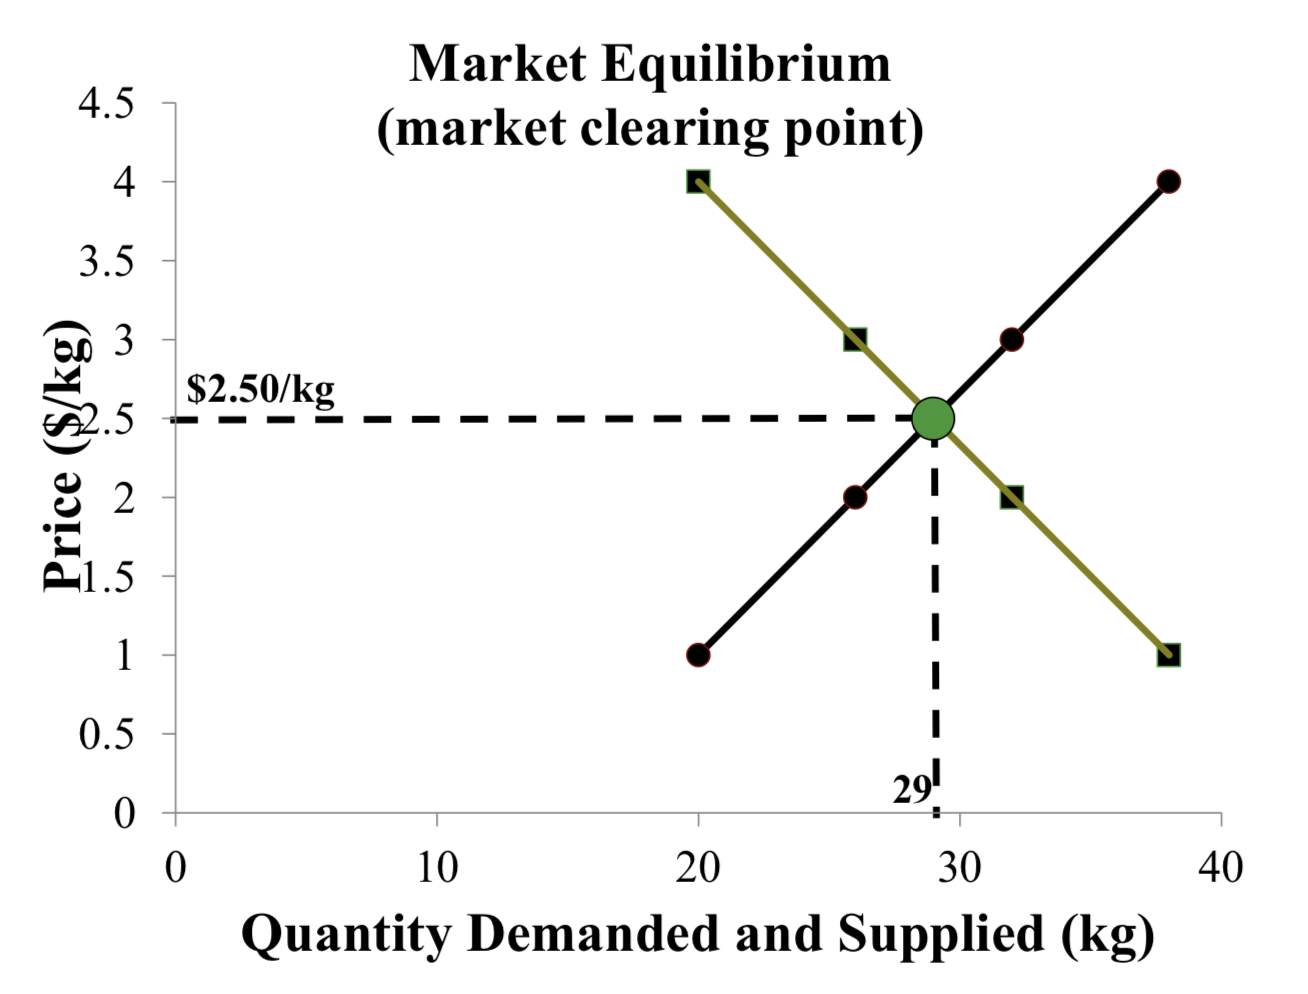
\includegraphics[width=0.9\linewidth]{cross}
	\caption{Market Equilibrium}
\end{figure}
\begin{itemize}
	\item The intersection of the supply and demand curves so $\rightarrow$ quantity supplied = quantity demanded AND selling price = purchase price
	\item A point where suppliers are happy to sell a given quantity at a certain price, and this exactly matches the price consumers are willing to  pay for this quantity supplied
\end{itemize}

\subsection{Market Clearing Point}
\subsubsection{Competitive Market}
\begin{itemize}
	\item has many buyers and many sellers
	\item Prices and quantities continue to adjust until a market clearning point is reached, eliminating shortages and surpluses
	\item note the market clearing point and the \textbf{model suggests} equilibrium is a \textbf{static point}. In reality, it can continually move. i.e. the point is \textbf{dynamic}
\end{itemize}
\begin{description}
	\item[Price Floor:] Price can be set higher than market clearing
	\item[Price Ceiling:] Price can be set lower than market clearing
\end{description}
\subsubsection{Price Floor}
\begin{itemize}
	\item used by governments to set a legally determined price to protect suppliers
	\item the price is set \textbf{above} the market clearing price, and becomes a minimum price for suppliers
	\item this minimum price is then guaranteed by the government
\end{itemize}
\subsubsection{Price Ceiling}
\begin{itemize}
	\item used by governments to set a legally determined price to protect consumers (e.g. tenants who rent, petrol ``price caps'' when oil prices rising fast)
	\item the price is set \textbf{below} the market clearning price, to help protect consumers from higher prices
	\item the legal price is a maximum that can be charged by suppliers
	\item What about \textbf{illegally} paying higher prices for the quantity that \textbf{is} available? \textbf{Black Markets}?
\end{itemize}
\textbf{Market Failure:} an inefficient allocation of goods and services in a market

\begin{figure}[H]
	\centering
	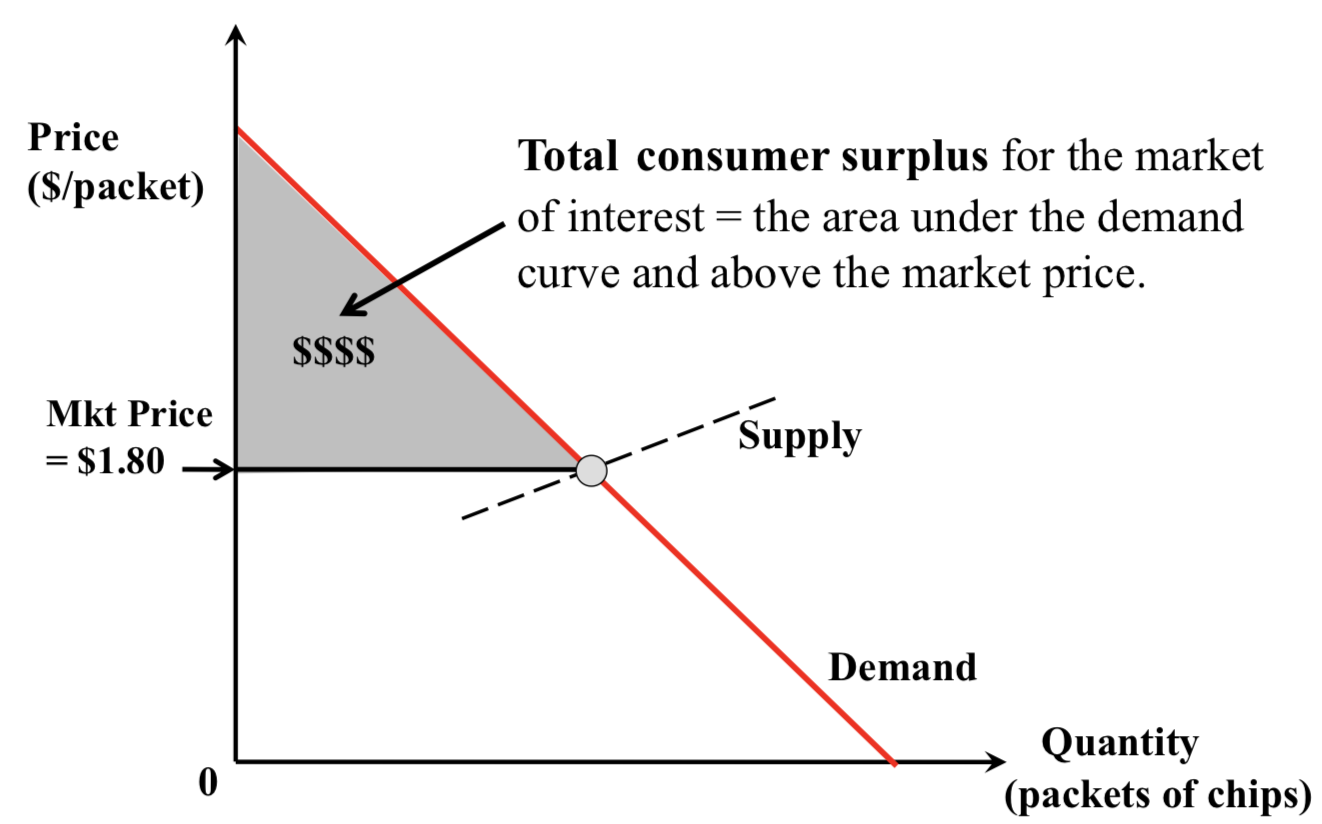
\includegraphics[width=0.9\linewidth]{consumerSurplus}
	\caption{Total Consumer Surplus}\label{fig:consumer}
\end{figure}
\begin{note}{Consumer Surplus}
	The maximum price an individual consumer is prepared to pay less the clearing price set by the market = an individual's consumer surplus.\\
	See Figure~\ref{fig:consumer}
\end{note}
\begin{figure}[H]
	\centering
	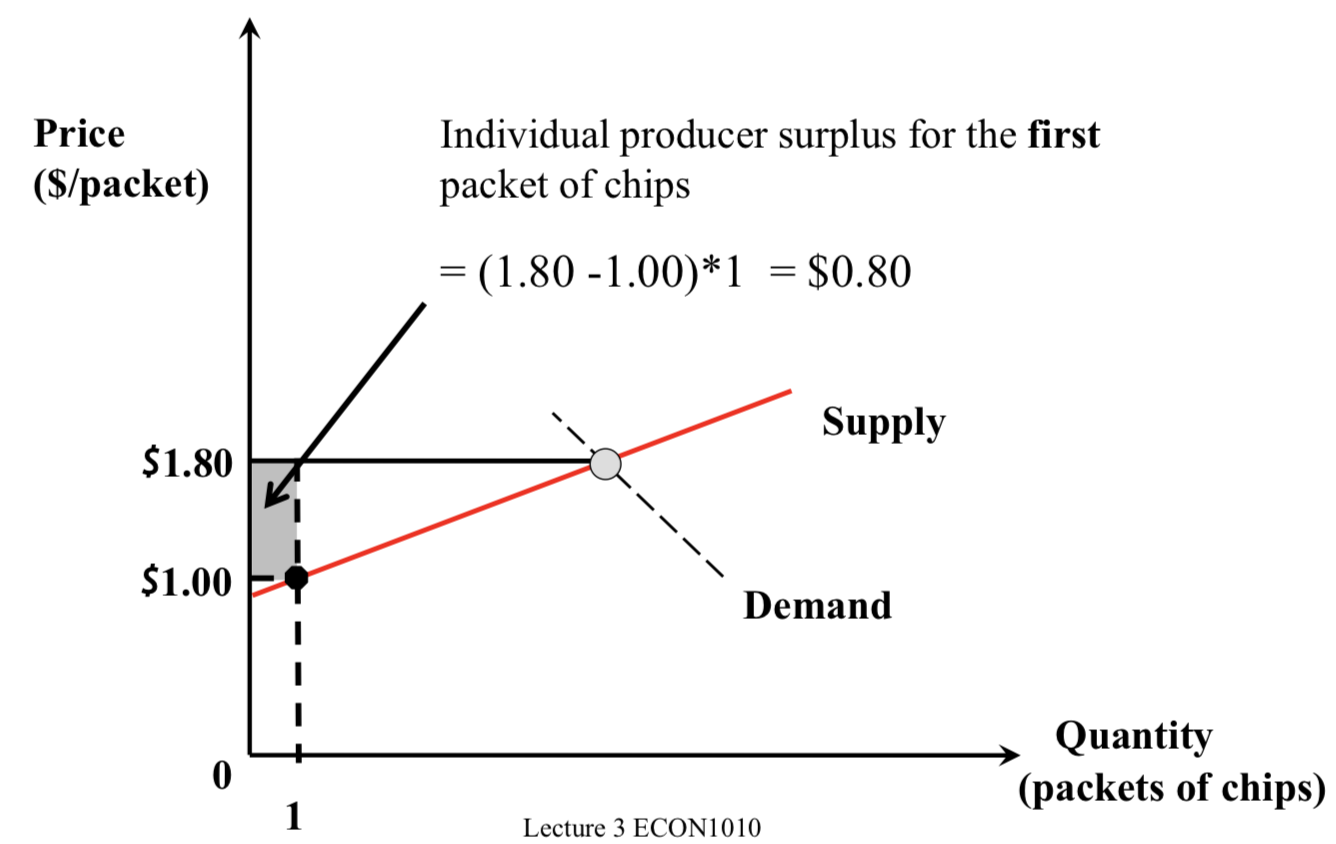
\includegraphics[width=0.9\linewidth]{producerSurplus}
	\caption{Individual Producer Surplus}\label{fig:producer}
\end{figure}
\begin{note}{Producer Surplus}
	The market clearing price less the minimum price a supplier would have been willing to accept in a sale\\
	See Figure~\ref{fig:producer}
\end{note}
\begin{note}{Economic Surplus}
	Total Economic Surplus = total consumer surplus + total producer surplus (maximised in competitive markets)
\end{note}
\subsubsection{Dead Weight Loss}
Economic inefficiency from government intervention. It's the area between the lines that is loss by introducing a Price Floor